\chapter{Flexion gauche}
La flexion gauche, ou oblique, consiste simplement en une combinaison de 
deux flexions simples.
\section{Théorie}
	\subsection{Flexions autour des deux axes}
	Précisons avant tout que l'on travaille \textbf{en axes principaux !} 
	Sans quoi, il n'y a pas de séparation selon les axes\footnote{Il est 
	préférable de travailler avec $C_y,C_z$ en 3D pour éviter les 
	conventions de signe de $M_y,M_z,\dots$.}. Considérons nos deux 
	flexions :
	\begin{equation}
	\begin{array}{lll}
	\text{Autour de l'axe $z$ : } & \sigma_x &= -\dfrac{C_z}{I_z}y\\
	\text{Autour de l'axe $y$ : } & \sigma_x &= \dfrac{C_y}{I_y}z	
	\end{array}
	\end{equation}
	En additionnant :
	\begin{equation}
	\displaystyle	\sigma_x = -\dfrac{C_z}{I_z}y + \dfrac{C_y}{I_y}z
	\end{equation}

	\subsection{A la recherche de l'axe neutre}
	De façon plus visuelle, nous venons de faire l'opération suivante : 
	\begin{center}
	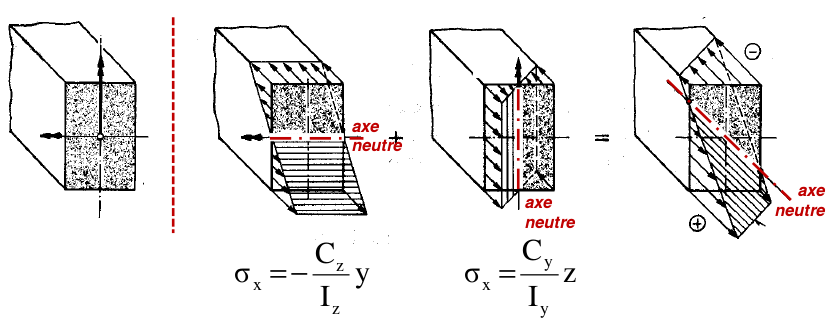
\includegraphics[scale=0.4]{ch6/image1.png}
	\captionof{figure}{ }
	\end{center}
	L'équation de l'axe neutre est alors 
	\begin{equation}
	\sigma_x = 0\qquad \Longrightarrow -\dfrac{C_z}{I_z}y + \dfrac{C_y
	}{I_y}z=0
	\end{equation}
	\danger Encore une fois, il faut travailler dans les axes principaux 
	de la section !